\documentclass[tikz,border=8pt]{standalone}
\usepackage[T1]{fontenc}
\usepackage{lmodern}
\usepackage{tikz}
\usetikzlibrary{arrows.meta,positioning,calc}

\begin{document}
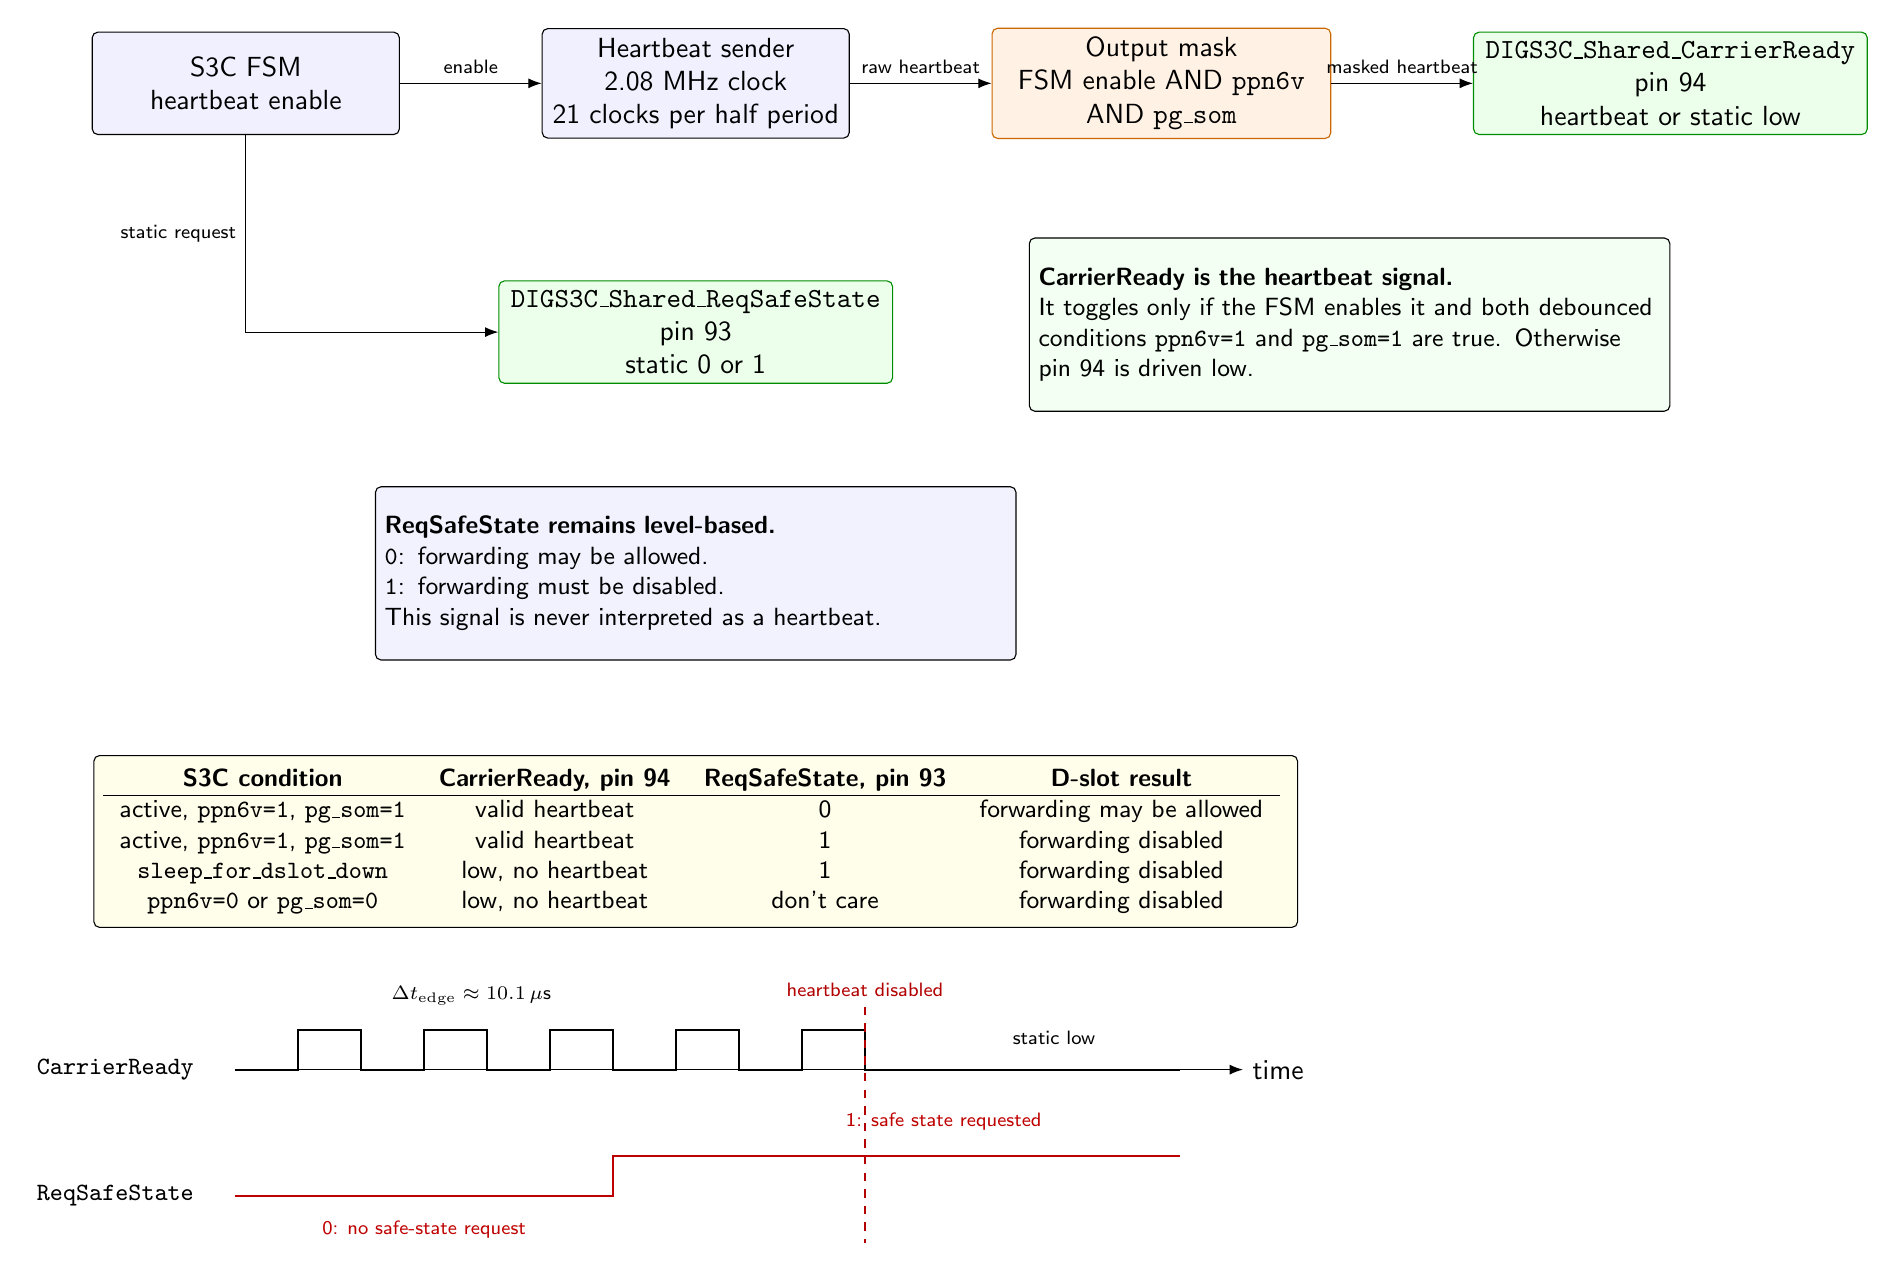
\begin{tikzpicture}[
  font=\sffamily,
  >=Latex,
  block/.style={draw, rounded corners=2pt, align=center, minimum height=13mm,
                minimum width=39mm, fill=blue!6},
  gate/.style={draw=orange!80!black, rounded corners=2pt, align=center,
               minimum height=13mm, minimum width=43mm, fill=orange!10},
  signal/.style={draw=green!55!black, rounded corners=2pt, align=center,
                 minimum height=13mm, minimum width=50mm, fill=green!8},
  info/.style={draw, rounded corners=2pt, align=left, font=\sffamily\small,
               text width=79mm, minimum height=22mm},
  note/.style={font=\sffamily\small, align=center},
  tiny/.style={font=\sffamily\scriptsize, align=center},
  sig/.style={thick}
]

% S3C sender path
\node[block] (fsm) {S3C FSM\\heartbeat enable};
\node[block, right=18mm of fsm] (sender)
  {Heartbeat sender\\2.08 MHz clock\\21 clocks per half period};
\node[gate, right=18mm of sender] (mask)
  {Output mask\\FSM enable AND \texttt{ppn6v}\\AND \texttt{pg\_som}};
\node[signal, right=18mm of mask] (carrier)
  {\texttt{DIGS3C\_Shared\_CarrierReady}\\pin 94\\heartbeat or static low};

\draw[->] (fsm) -- node[above,tiny] {enable} (sender);
\draw[->] (sender) -- node[above,tiny] {raw heartbeat} (mask);
\draw[->] (mask) -- node[above,tiny] {masked heartbeat} (carrier);

% Independent static safe-state path
\node[signal, below=18mm of sender] (reqsafe)
  {\texttt{DIGS3C\_Shared\_ReqSafeState}\\pin 93\\static 0 or 1};
\draw[->] (fsm.south) |- node[pos=.25,left,tiny] {static request} (reqsafe.west);

% Explanations
\node[info, fill=green!5, below=13mm of carrier, anchor=north east] (carrierinfo) {
  \textbf{CarrierReady is the heartbeat signal.}\\
  It toggles only if the FSM enables it and both debounced conditions
  \texttt{ppn6v=1} and \texttt{pg\_som=1} are true.
  Otherwise pin 94 is driven low.
};

\node[info, fill=blue!5, below=13mm of reqsafe, anchor=north] (safeinfo) {
  \textbf{ReqSafeState remains level-based.}\\
  \texttt{0}: forwarding may be allowed.\\
  \texttt{1}: forwarding must be disabled.\\
  This signal is never interpreted as a heartbeat.
};

% Truth table
\node[draw, rounded corners=2pt, fill=yellow!8, align=center,
      font=\sffamily\small, below=12mm of safeinfo, anchor=north] (table) {
\begin{tabular}{c c c c}
\textbf{S3C condition} & \textbf{CarrierReady, pin 94}
& \textbf{ReqSafeState, pin 93} & \textbf{D-slot result}\\
\hline
active, \texttt{ppn6v=1}, \texttt{pg\_som=1}
& valid heartbeat & 0 & forwarding may be allowed\\
active, \texttt{ppn6v=1}, \texttt{pg\_som=1}
& valid heartbeat & 1 & forwarding disabled\\
\texttt{sleep\_for\_dslot\_down}
& low, no heartbeat & 1 & forwarding disabled\\
\texttt{ppn6v=0} or \texttt{pg\_som=0}
& low, no heartbeat & don't care & forwarding disabled
\end{tabular}
};

% Compact timing example
\coordinate (t0) at ($(table.south west)+(18mm,-18mm)$);
\draw[->] (t0) -- ++(128mm,0) node[right] {time};
\node[note, anchor=east] at ($(t0)+(-4mm,0mm)$)
  {\texttt{CarrierReady}};
\node[note, anchor=east] at ($(t0)+(-4mm,-16mm)$)
  {\texttt{ReqSafeState}};

% CarrierReady: heartbeat, then disabled low.
\draw[sig] ($(t0)+(0,0)$)
  -- ++(8mm,0) -- ++(0,5mm) -- ++(8mm,0) -- ++(0,-5mm)
  -- ++(8mm,0) -- ++(0,5mm) -- ++(8mm,0) -- ++(0,-5mm)
  -- ++(8mm,0) -- ++(0,5mm) -- ++(8mm,0) -- ++(0,-5mm)
  -- ++(8mm,0) -- ++(0,5mm) -- ++(8mm,0) -- ++(0,-5mm)
  -- ++(8mm,0) -- ++(0,5mm) -- ++(8mm,0) -- ++(0,-5mm)
  -- ++(40mm,0);
\draw[dashed, red!70!black] ($(t0)+(80mm,8mm)$) -- ($(t0)+(80mm,-22mm)$);
\node[tiny, red!70!black, anchor=south] at ($(t0)+(80mm,8mm)$)
  {heartbeat disabled};
\node[tiny, anchor=south] at ($(t0)+(30mm,7mm)$)
  {$\Delta t_{\mathrm{edge}}\approx10.1\,\mu$s};
\node[tiny, anchor=south] at ($(t0)+(104mm,2mm)$) {static low};

% ReqSafeState: independent static request.
\draw[sig, red!75!black] ($(t0)+(0,-16mm)$) -- ++(48mm,0)
  -- ++(0,5mm) -- ++(72mm,0);
\node[tiny, red!75!black, anchor=north] at ($(t0)+(24mm,-18mm)$)
  {0: no safe-state request};
\node[tiny, red!75!black, anchor=south] at ($(t0)+(90mm,-9mm)$)
  {1: safe state requested};

\end{tikzpicture}
\end{document}
